\documentclass[11pt,a4paper]{article}

\usepackage[utf8]{inputenc}
\usepackage[T1]{fontenc}
\usepackage[margin=2.2cm]{geometry}
\usepackage{xcolor}
\usepackage{titlesec}
\usepackage{enumitem}
\usepackage{listings}
\usepackage{hyperref}
\usepackage{fancyhdr}
\usepackage{parskip}
\usepackage[protrusion=true,expansion=false]{microtype}
\usepackage{tikz}
\usepackage{tcolorbox}
\usepackage{array}
\usepackage{booktabs}
\usepackage{graphicx}
\tcbuselibrary{breakable, skins}

\definecolor{nearblack}{HTML}{0A0A0A}
\definecolor{offwhite}{HTML}{FAFAF7}
\definecolor{mutedgrey}{HTML}{6B6B6B}
\definecolor{hairline}{HTML}{D4D4D4}
\definecolor{codebg}{HTML}{F4F4F0}
\definecolor{accent}{HTML}{1A1A1A}

\hypersetup{
    colorlinks=true,
    linkcolor=nearblack,
    urlcolor=accent,
    pdftitle={Job Tracker --- README},
    pdfauthor={Unc}
}

\pagestyle{fancy}
\fancyhf{}
\renewcommand{\headrulewidth}{0pt}
\fancyfoot[L]{\small\color{mutedgrey}\textsc{Job Tracker --- README}}
\fancyfoot[R]{\small\color{mutedgrey}\thepage}

\titleformat{\section}
  {\normalfont\Large\bfseries\color{nearblack}}
  {\color{mutedgrey}\ttfamily\small\thesection\quad}{0pt}{}
  [\vspace{2pt}{\color{hairline}\hrule height 0.4pt}]

\titleformat{\subsection}
  {\normalfont\large\bfseries\color{nearblack}}
  {\color{mutedgrey}\ttfamily\footnotesize\thesubsection\quad}{0pt}{}

\titlespacing*{\section}{0pt}{20pt}{8pt}
\titlespacing*{\subsection}{0pt}{14pt}{4pt}

\lstdefinestyle{codeblock}{
  backgroundcolor=\color{codebg},
  basicstyle=\ttfamily\footnotesize\color{nearblack},
  commentstyle=\color{mutedgrey}\itshape,
  keywordstyle=\color{nearblack}\bfseries,
  breaklines=true,
  breakatwhitespace=true,
  showstringspaces=false,
  frame=single,
  framerule=0.3pt,
  rulecolor=\color{hairline},
  xleftmargin=10pt,
  xrightmargin=10pt,
  framexleftmargin=8pt,
  framexrightmargin=8pt,
  aboveskip=10pt,
  belowskip=10pt,
  columns=fullflexible,
  keepspaces=true,
  upquote=true,
}
\lstset{style=codeblock}

\newtcolorbox{callout}[1][]{
  enhanced,
  breakable,
  colback=offwhite,
  colframe=hairline,
  boxrule=0.4pt,
  arc=0pt,
  outer arc=0pt,
  left=10pt, right=10pt, top=8pt, bottom=8pt,
  fonttitle=\bfseries\small,
  coltitle=nearblack,
  title={#1},
  attach boxed title to top left={xshift=8pt, yshift=-7pt},
  boxed title style={
    colback=offwhite,
    colframe=offwhite,
    arc=0pt,
    outer arc=0pt,
    boxrule=0pt,
    left=4pt, right=4pt, top=0pt, bottom=0pt,
  },
  top=14pt,
}

\newcommand{\imgplaceholder}[1]{%
  \begin{center}
  \tikz{\draw[draw=hairline,line width=0.4pt,fill=codebg] 
    (0,0) rectangle (\linewidth,3.2);
    \node[mutedgrey] at (0.5\linewidth,1.6) 
      {\itshape\small [ #1 ]};}
  \end{center}
}

\setlist[itemize]{leftmargin=1.2em, itemsep=3pt, topsep=4pt}

\begin{document}

\thispagestyle{empty}
\vspace*{2cm}

{\color{mutedgrey}\ttfamily\small PORTFOLIO PROJECT --- README}

\vspace{6pt}
{\color{hairline}\hrule height 0.4pt}
\vspace{18pt}

{\fontsize{32}{36}\selectfont\bfseries\color{nearblack} Job Tracker}

\vspace{10pt}
{\Large\color{mutedgrey}\itshape A job application tracker built to be
used, not just demoed}

\vspace{20pt}
{\color{hairline}\hrule height 0.4pt}

\vspace{14pt}
\begin{minipage}{0.48\textwidth}
\color{mutedgrey}\small
\textsc{Links}\\[2pt]
\color{nearblack}
Live demo --- \texttt{[ url ]}\\
Repository --- \texttt{[ url ]}\\
Project write-up --- \texttt{[ url ]}
\end{minipage}
\begin{minipage}{0.48\textwidth}
\color{mutedgrey}\small
\textsc{Stack}\\[2pt]
\color{nearblack}
Next.js 14, Supabase\\
Tailwind + shadcn/ui\\
DistilBERT, Modal\\
Deployed on Vercel
\end{minipage}

\vspace{1.6cm}
\begin{center}
  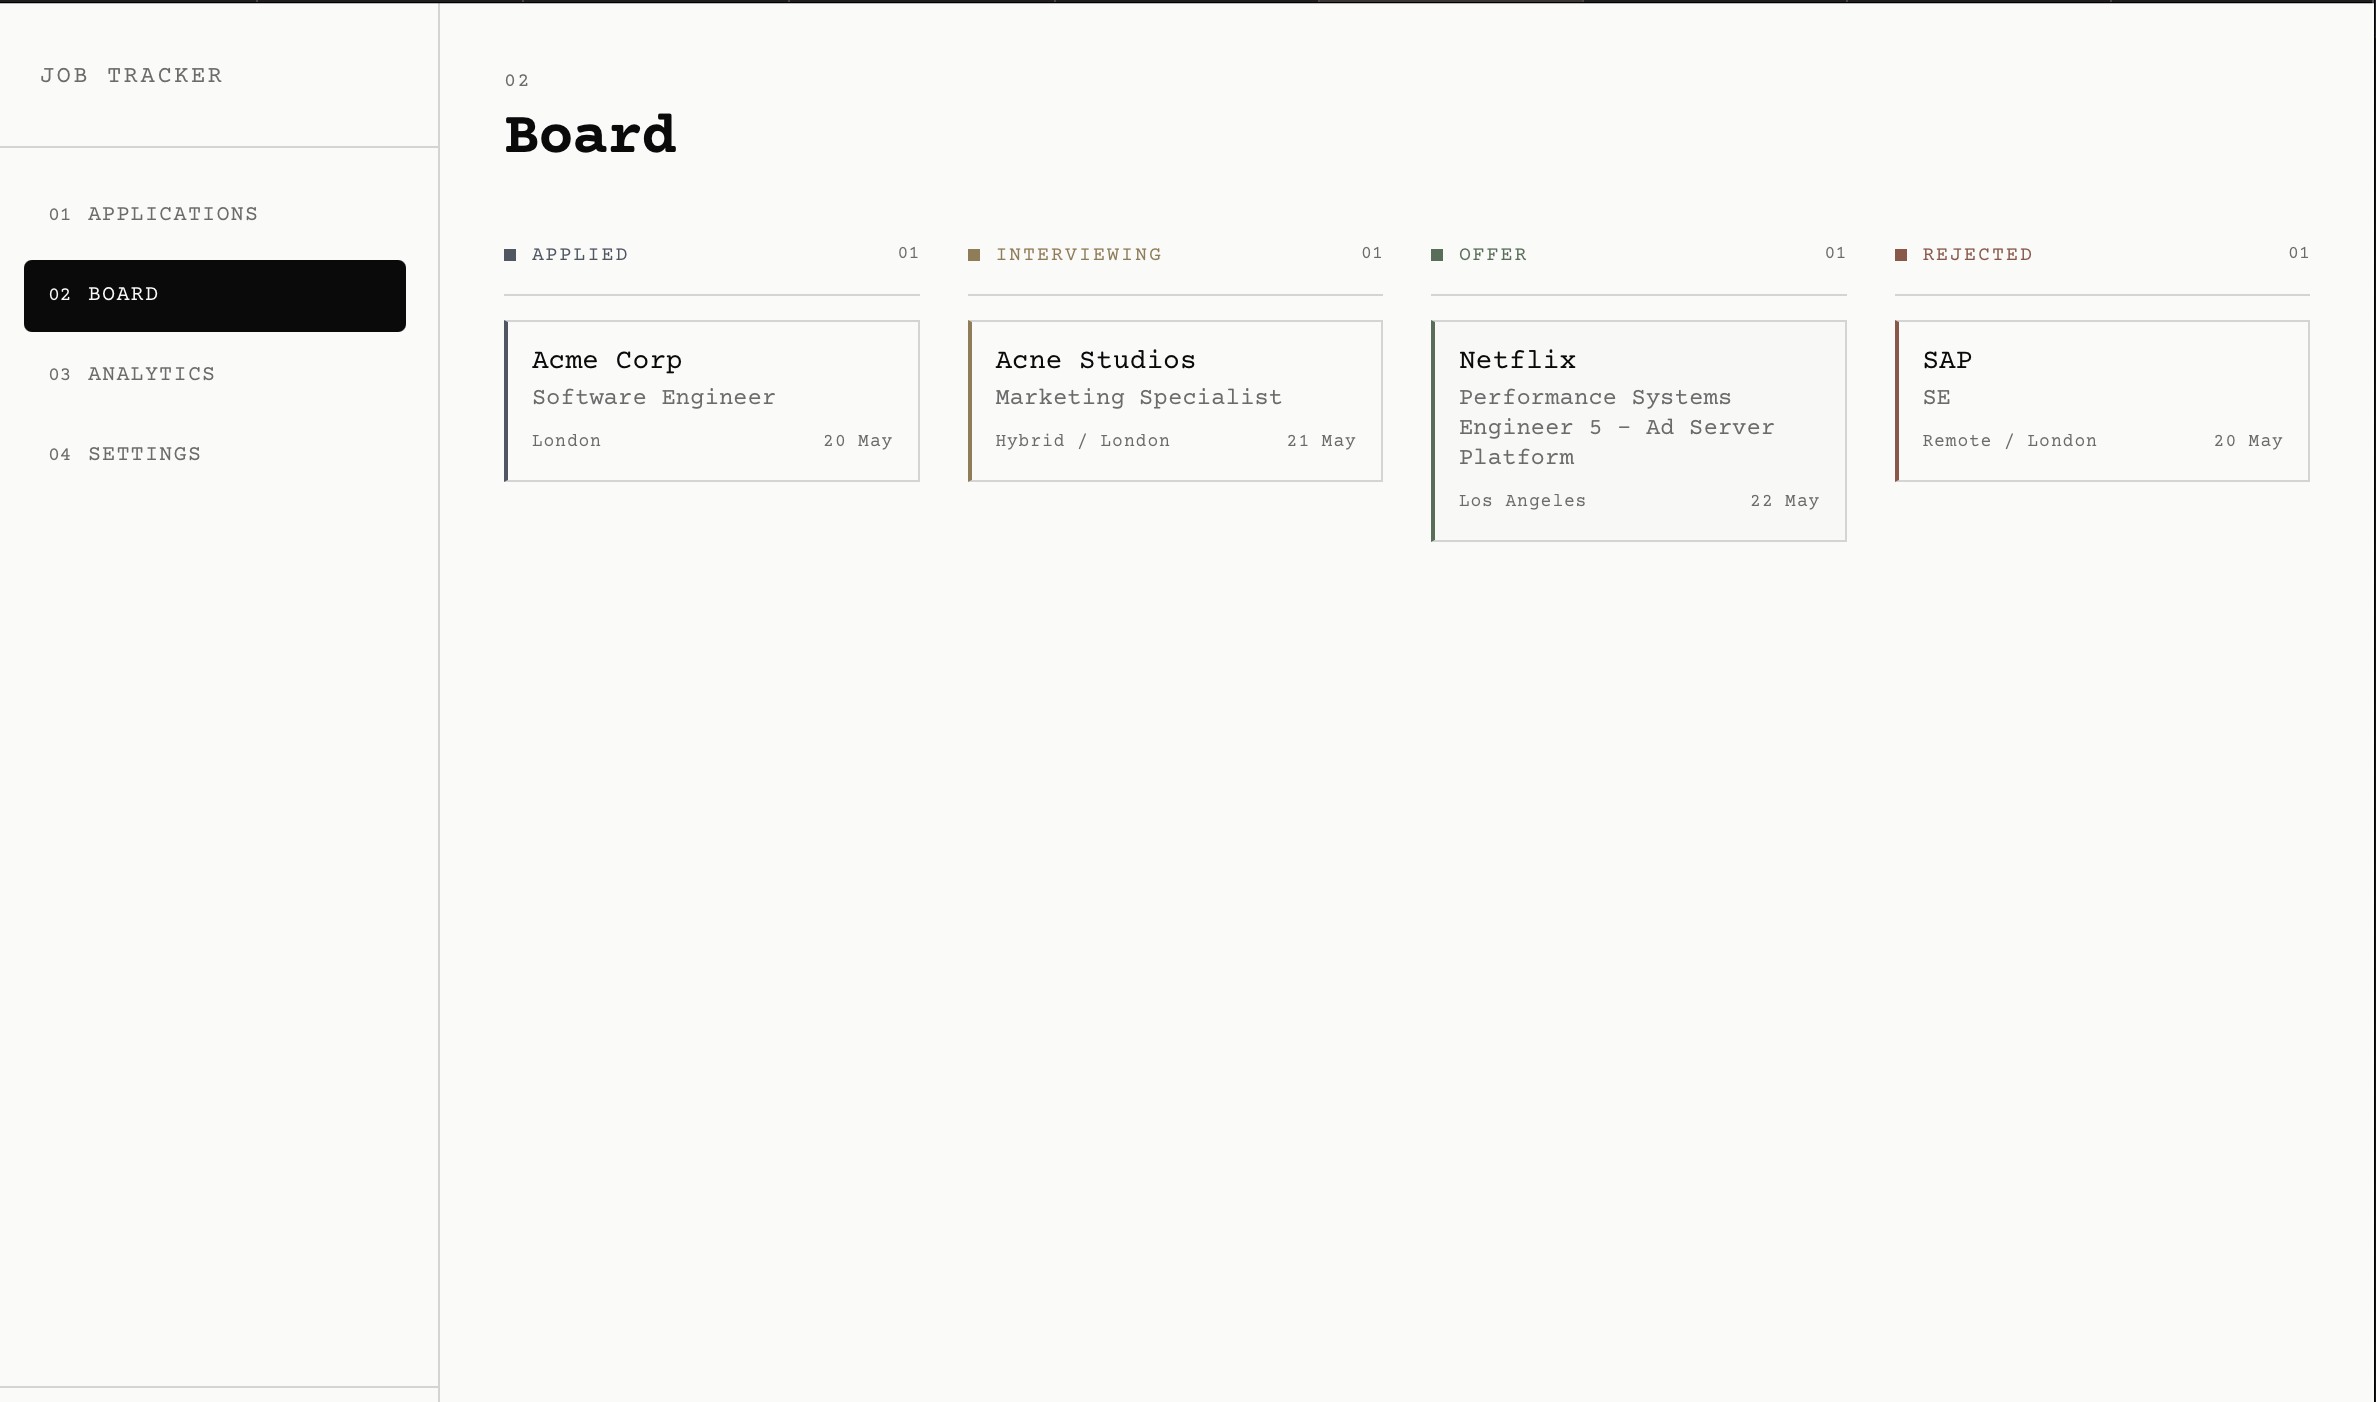
\includegraphics[width=\linewidth]{Images/1HERO.png}
\end{center}

\vspace{0.6cm}

\newpage

% =============================================================
\section{Why This Exists}

I was tracking job applications in a spreadsheet and it was doing the job
badly. No sense of pipeline, and a lot of repetitive data entry every time I found a posting. 
So I built the tool I actually wanted. Something that shows the shape of a job search and
removes the tedious parts of logging an application.

It's also a portfolio project, so a second goal ran alongside the first.
Build something that demonstrates real full-stack and my own introduction to ML work. 

% =============================================================
\section{Stack}

\begin{itemize}
  \item \textbf{Next.js 14} (App Router): server components, server actions
  \item \textbf{Supabase}: Postgres, authentication, RLS
  \item \textbf{Tailwind CSS + shadcn/ui}: styling and component primitives
  \item \textbf{DistilBERT} (fine-tuned): named entity extraction for the URL parser
  \item \textbf{Modal}: stz hosting for the ML inference endpoint
  \item \textbf{Vercel}: deployment
\end{itemize}

% =============================================================
\section{Features}

\subsection{Applications (table view)}

Every application in a sortable table, which looks like this;  
company, role, status, applied date, location. Add and edit through a 
dialog with the full field set (salary range, job URL, notes). Delete asks for 
confirmation. A saved job URL opens in a new tab. Proper empty and loading states throughout.

\begin{center}
  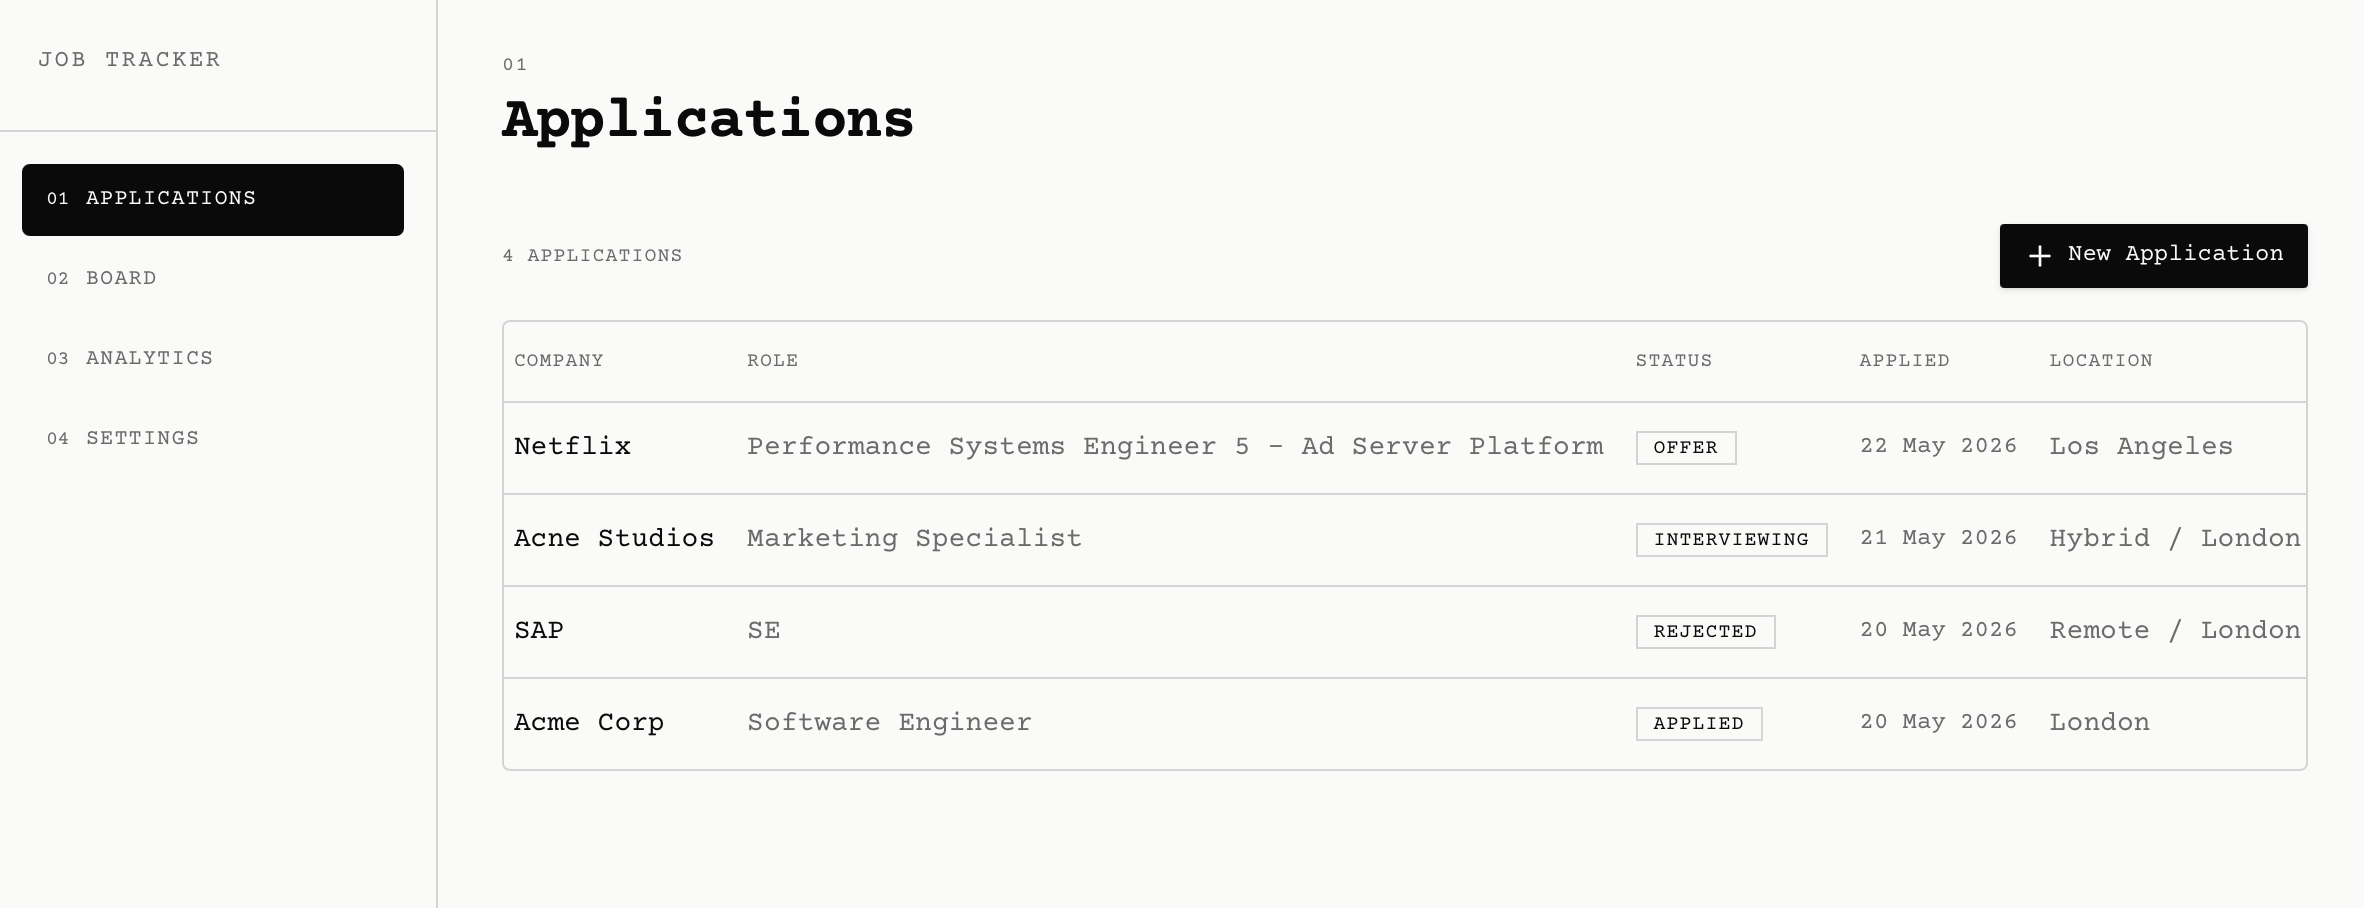
\includegraphics[width=\linewidth]{Images/2Tableview.png}
\end{center}

\subsection{Board (kanban view)}

Four columns: Applied, Interviewing, Offer, Rejected. Cards drag between
columns and their position persists. The UI updates, so the card moves 
immediately and only rolls back if the server rejects the change.

The board is the one view with colour. Each column carries a muted hue,
graphite, ochre, sage, rust, applied as a 2px left border on cards and
an accent on the column header. The hues were chosen for editorial
neutrality rather than traffic-light convention. Sage for offer instead
of bright green, rust for rejected instead of red. Every other view stays
black-and-white, which is what makes the colour on the board read as
deliberate.

\begin{center}
  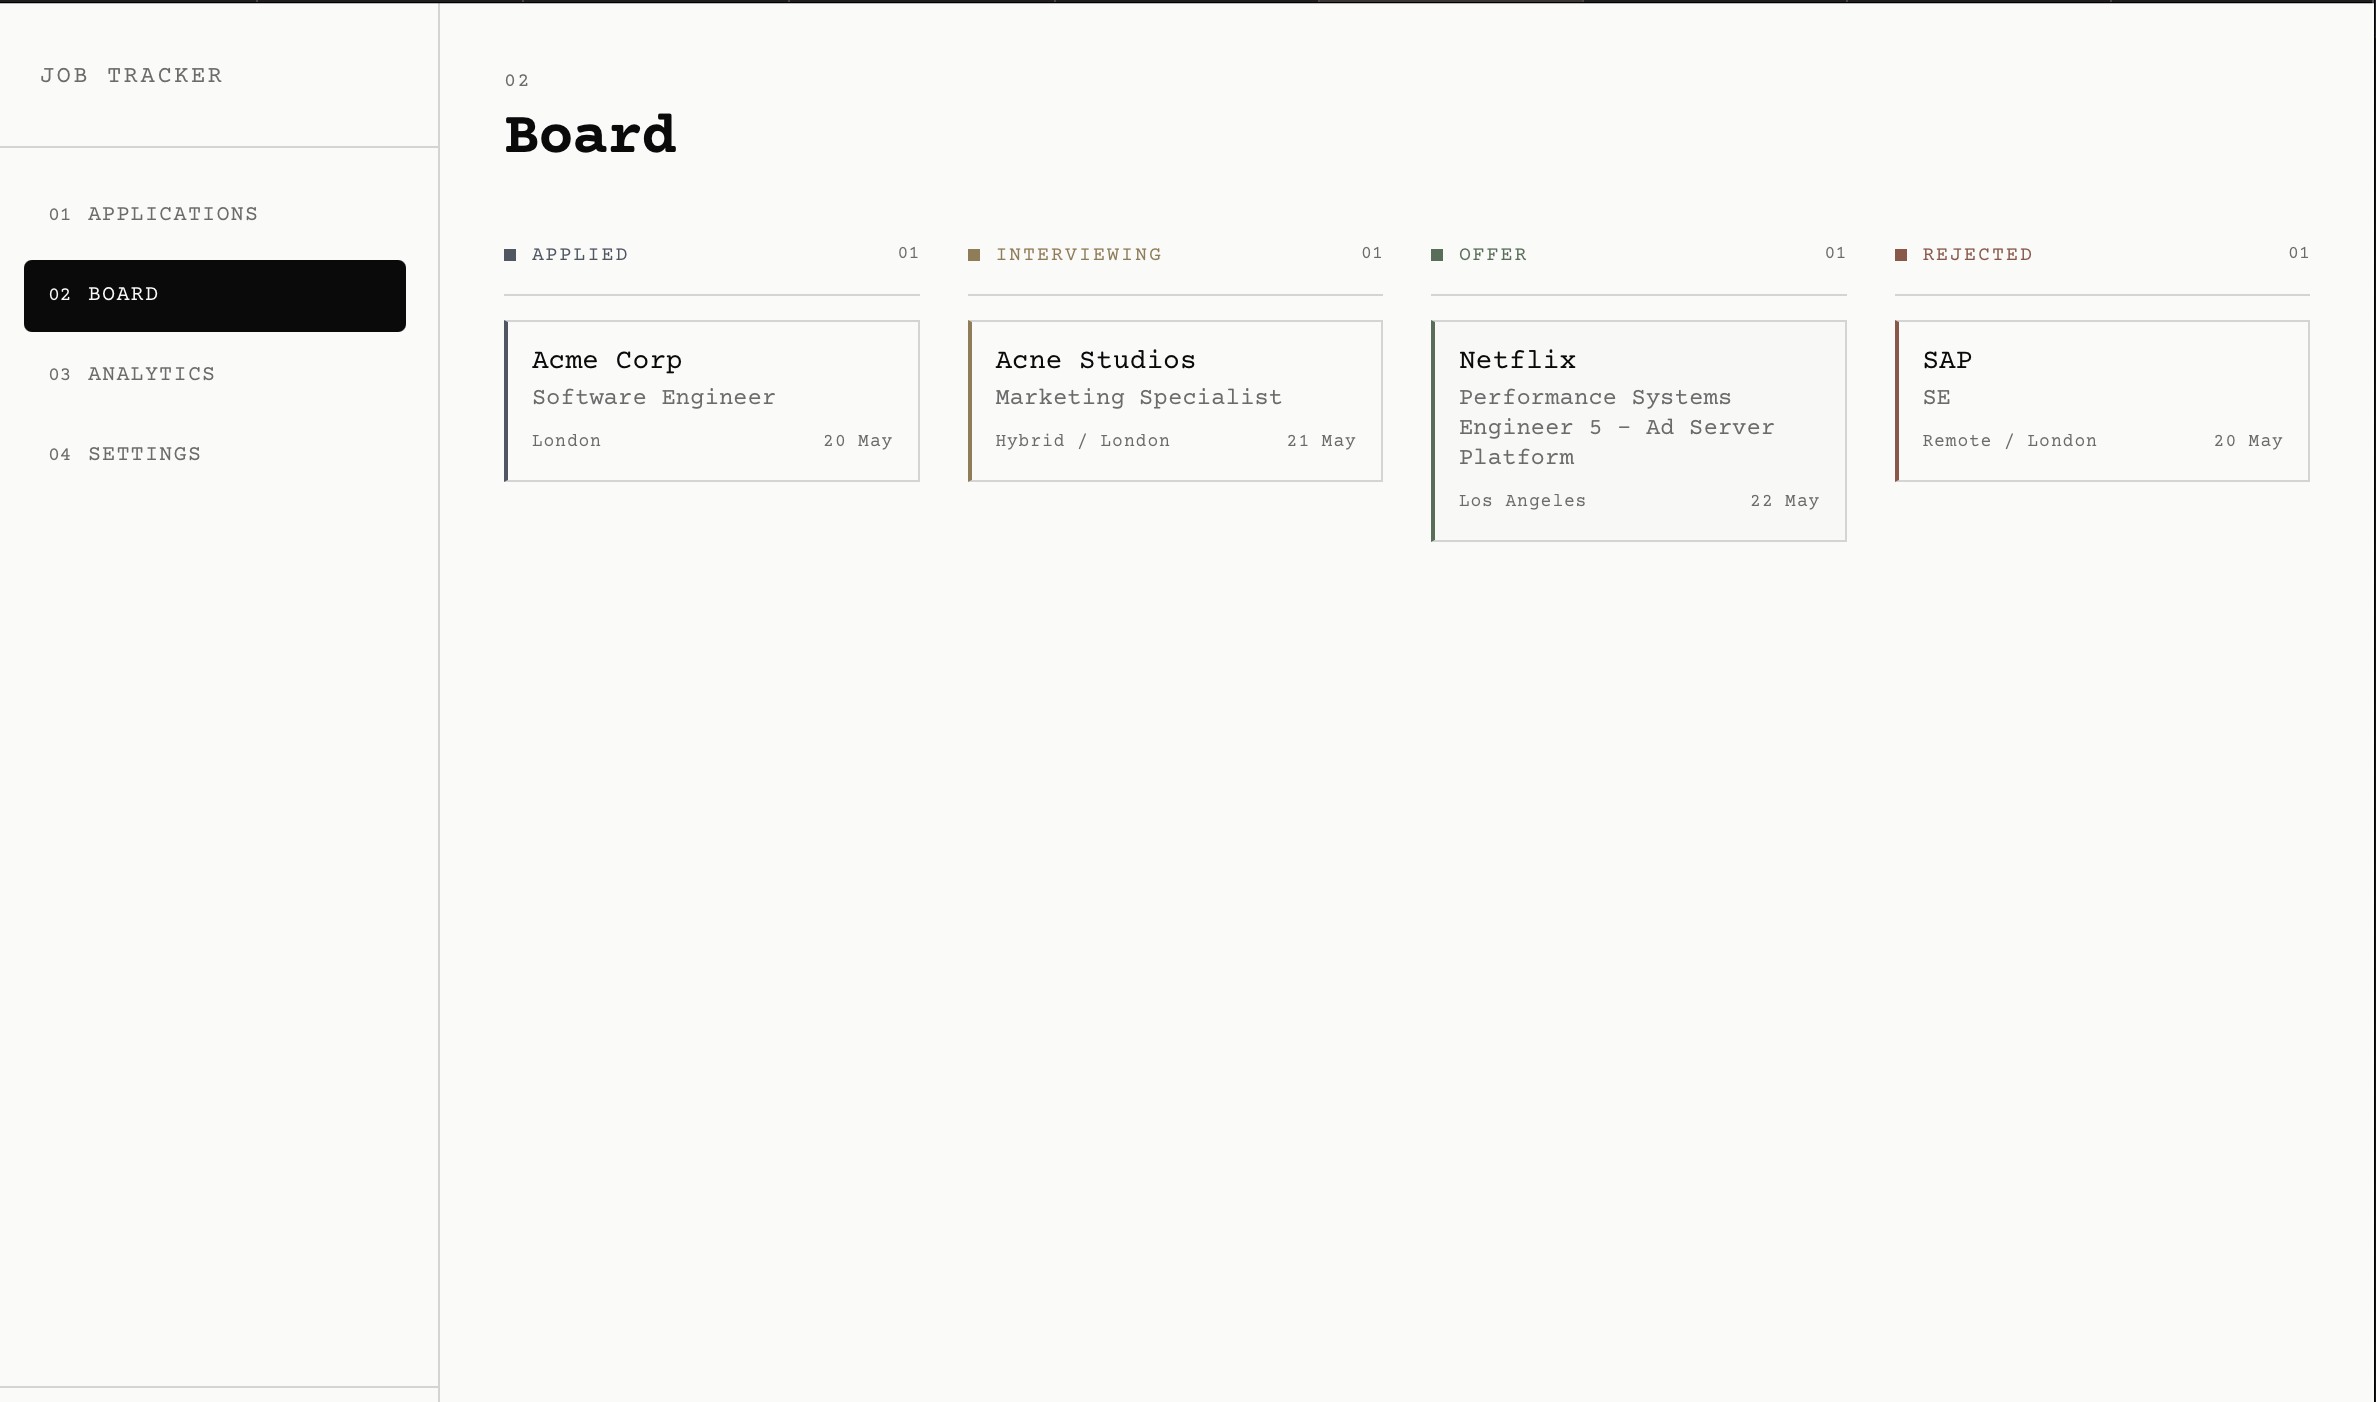
\includegraphics[width=\linewidth]{Images/3Hues copy.png}
\end{center}

\subsection{Analytics}

A dashboard that answers five questions: how many applications, how many
active in the pipeline, how many offers, application velocity, and stage
timing. A weekly line chart, a proportional funnel, and an average-days
breakdown between stages.

All the aggregation happens in Postgres via a view and two RPC functions,
not in application code. The database is the right layer for this work.
Faster, and it keeps the query logic in one place.

\begin{center}
  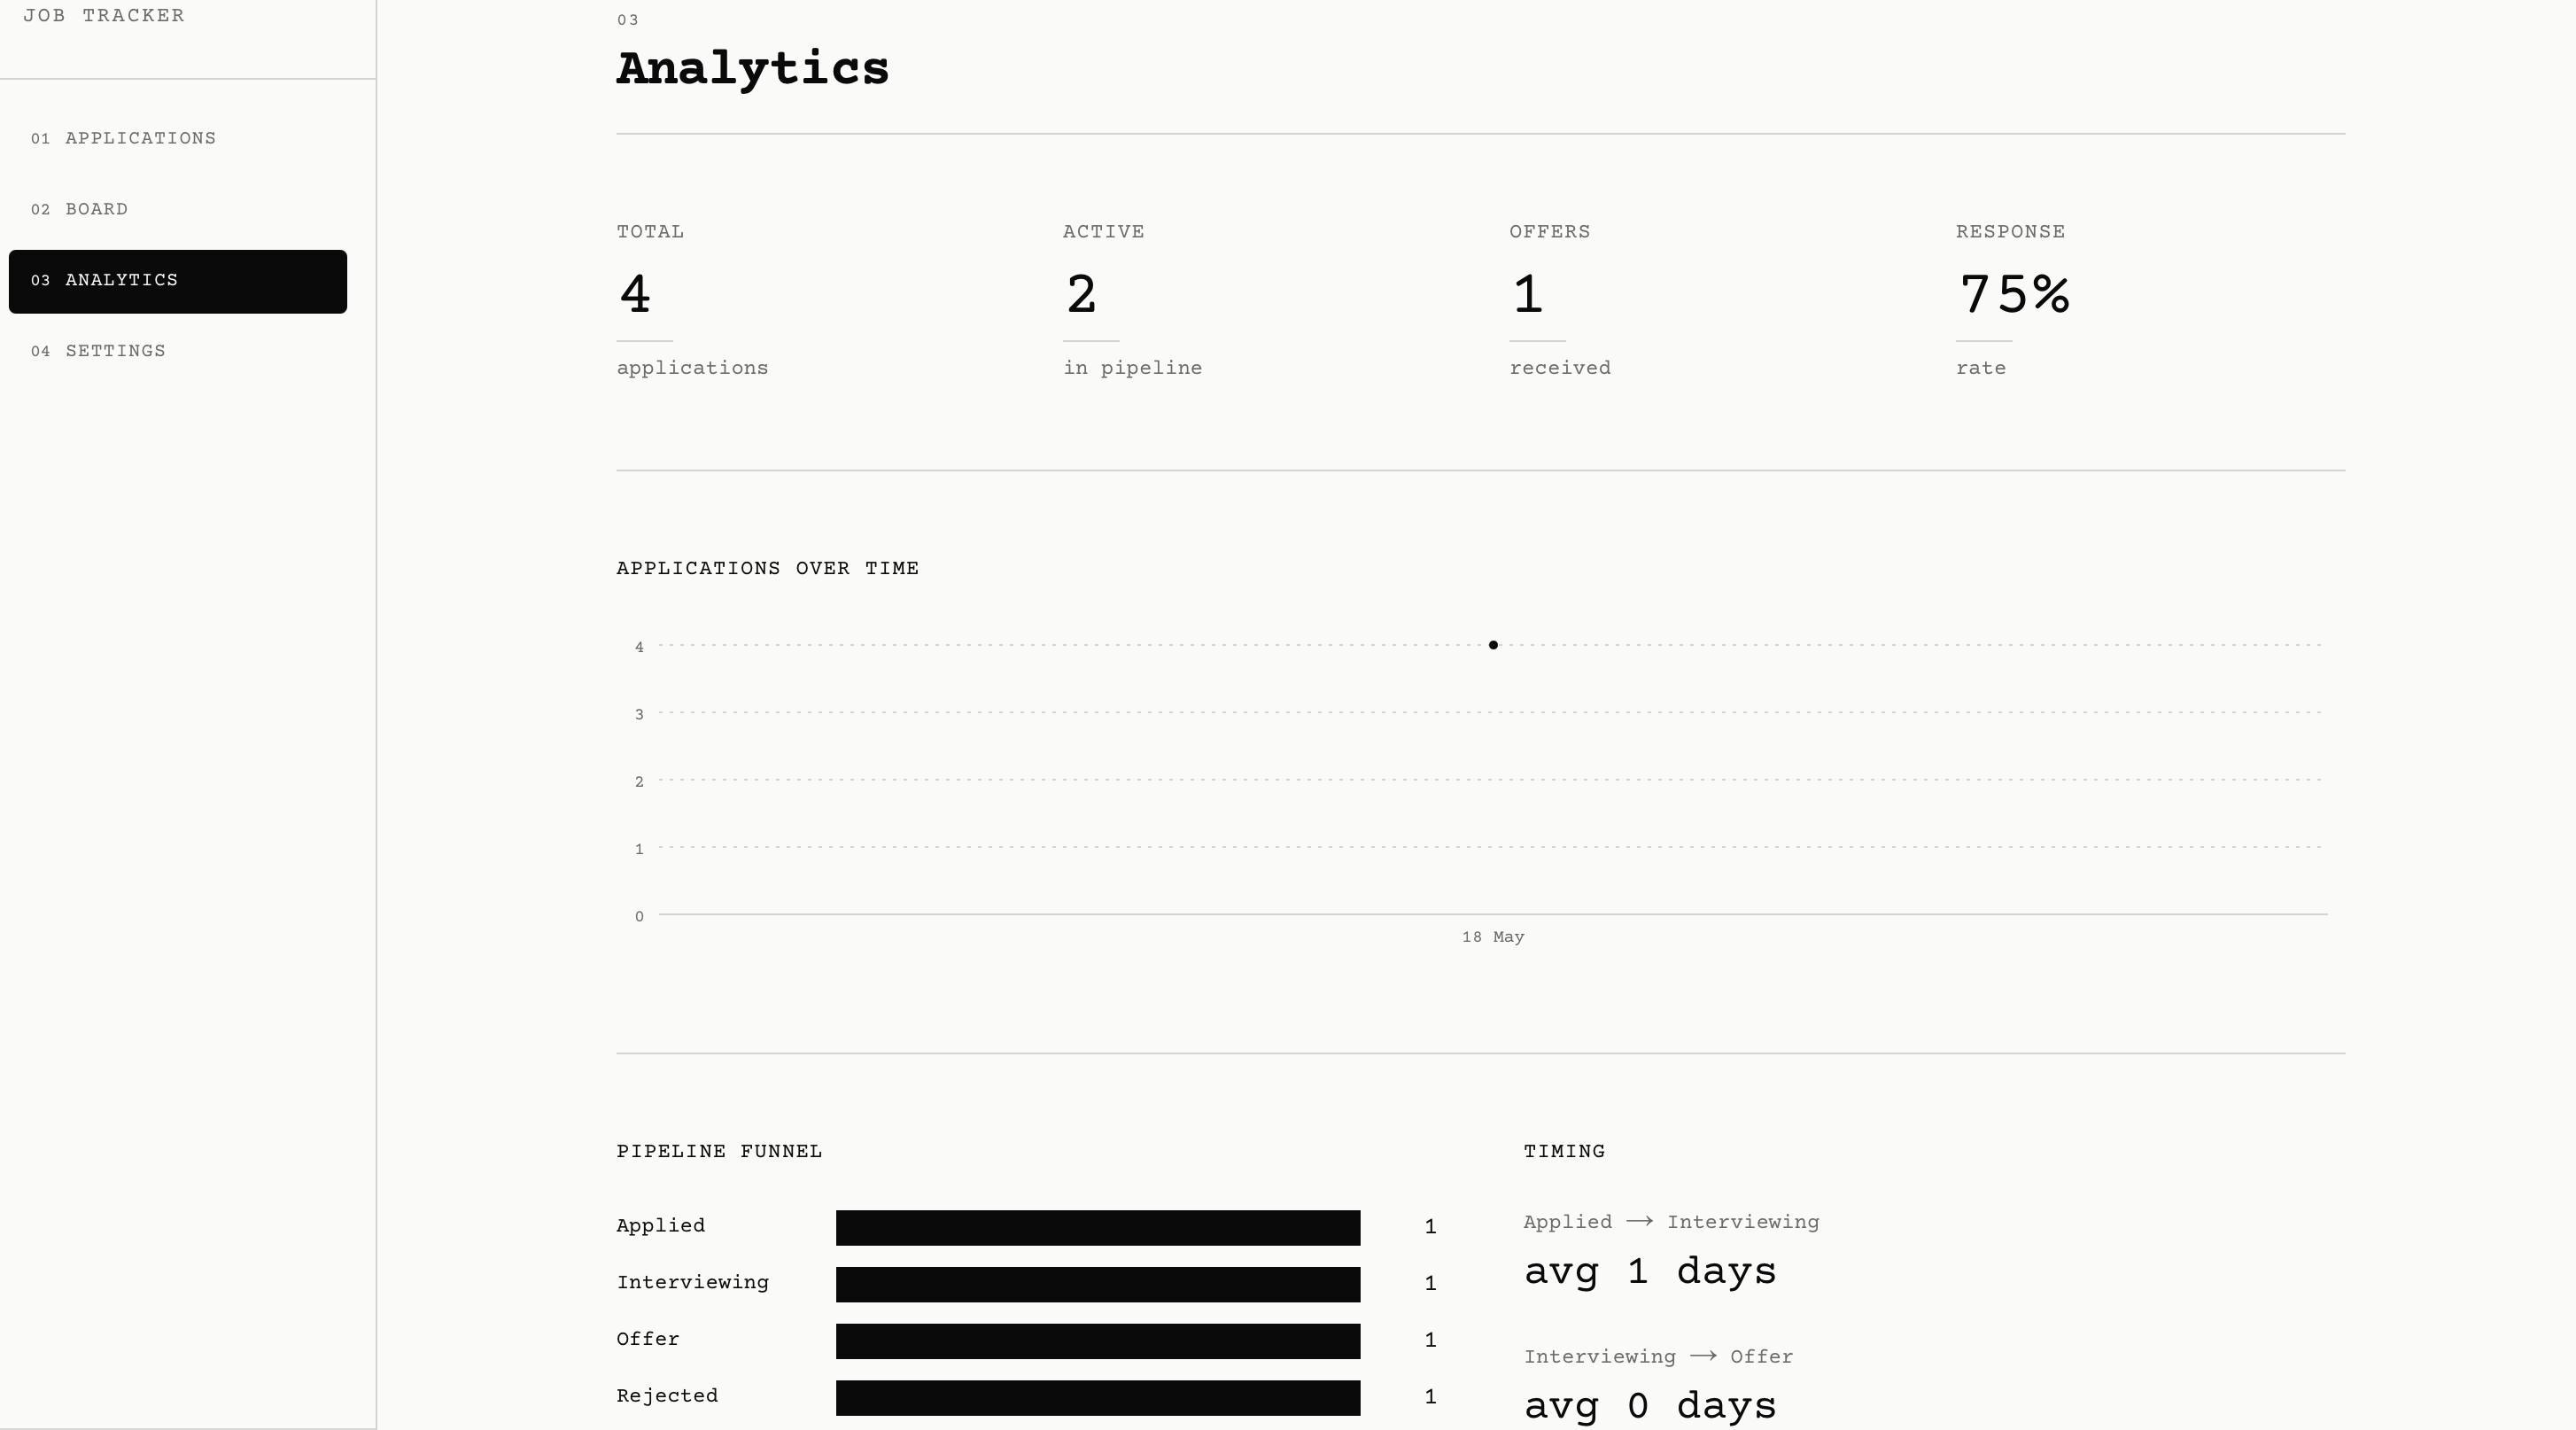
\includegraphics[width=\linewidth]{Images/4Analytics.png}
\end{center}

\subsection{AI job parser}

The feature I'm most pleased with. The new-application dialog has a
``quick fill'' row: paste a job URL, and the form pre-fills company, role,
location, and salary.

The pipeline does the cheap thing first. For Greenhouse and Lever URLs,
and for any page that exposes JSON-LD \texttt{JobPosting} structured data,
the fields are extracted directly from the HTML with CSS selectors, no
model involved. The fine-tuned model is the fallback for everything else.
A toast tells the user which path ran, so the tool is upfront about when
it is guessing.

LinkedIn, Indeed, and Workday are explicitly unsupported. They either
block scrapers or require JS rendering. These return a clear error rather
than failing silently.

\imgplaceholder{GIF: paste a URL, watch the fields populate}

\subsection{Settings and dark mode}

Profile and password management, a default-view preference, JSON and CSV
export, and a danger zone for deleting data or the whole account
(destructive actions require typing a confirmation phrase). Full dark
mode, warm off-white on near-black, designed rather than auto-inverted,
that syncs to the database so it follows the user accross devices.

% =============================================================
\section{The Machine Learning Piece}

The URL parser's fallback is a DistilBERT model fine-tuned for token
classification. It identifies five field types (company, role, location,
salary, employment type) using BIO tagging across 11 label classes.

\subsection{Dataset}

Training data was synthetic: 800 job postings generated with Claude, with
the field values fixed at generation time so the labels were known by
construction. This sidesteps the main cost of an NER dataset, which is
manual span labelling, while keeping the labels exact.

The validation set was real: 72 job postings hand-scraped from Greenhouse
and labelled by hand. Synthetic data is only useful if it generalises to
real postings, and the only way to know that is to measure against real
ones. 72 is a small set and I would grow it if I took this further, but
it was enough to show the model wasn't just memorising the synthetic
distribution.

\subsection{Deployment}

The model runs on Modal as a scale-to-zero FastAPI endpoint. No cost when
idle, a cold start of a few seconds on the first request, sub-two-second
inferance once warm. The Next.js app calls it server-side and the call is
rate-limited per user.

% =============================================================
\section{Security}

Security was treated as a feature. The notable
decisions:

\textbf{Authorization lives in the database.} RLS is
enabled on every table, so the database itself enforces that a user can
only ever read or write their own rows. A bug in the application layer
can't leak another user's data.

\textbf{RPC functions respect RLS.} The analytics aggregation functions
use \texttt{security invoker}, so they run with the caller's permissions
and RLS still applies. The one exception is the profile-creation trigger,
which uses \texttt{security definer} because it runs during signup, before
the user is authenticated.

\textbf{Input is never trusted.} Every server action validates its input
with Zod before touching the database. URL fields are validated as URLs,
which rejects \texttt{javascript:} pseudo-URLs, otherwise an XSS vector
on the ``open job listing'' button.

\textbf{Rate limiting is identifier-aware.} Auth endpoints are limited by
IP because the user isn't known yet. Authenticated actions are limited by
user ID. Limiting per-user actions by IP would let one user on a shared
network accidently rate-limit everyone else on it.

\textbf{Secrets stay server-side.} The admin client used for account
deletion imports the \texttt{server-only} package, so the build fails if
it ever gets pulled into client code. \texttt{gitleaks} was run over the
history before deploying.

HTTP security headers are set on every route. Custom 404 and error pages
replace the default Next.js ones.

% =============================================================
\section{What I Would Do Differently}

A few things I'd change:

\begin{itemize}
  \item \textbf{Stage timing is approximate.} The analytics ``average days
    between stages'' is computed from \texttt{applied\_at} and
    \texttt{updated\_at}, because the schema doesn't log per-stage
    transitions. A \texttt{status\_history} table would make this exact.
    It was a deliberate tradeoff, but it's the clearest piece of technical
    debt in the project.
  \item \textbf{The salary field underperforms}, for the reasons in the
    ML section above.
  \item \textbf{The validation set is small} at 72 examples. Enough to be
    indicative, not enough to be precise.
\end{itemize}

None of these block the tool from being genuinely useful, which was the
bar I set. 

\vspace{20pt}
{\color{hairline}\hrule height 0.4pt}
\vspace{12pt}

\begin{flushright}
\color{mutedgrey}\itshape\small
Canonical version: \texttt{README.md} in the repository.
\end{flushright}

\end{document}
